\documentclass[12pt]{article}
\usepackage{graphicx}

\begin{document}
\title{Notes for Reinforcement Learning for CAT Vehicle}
\maketitle

\section{Notes on Machine Learning for Autonomous Driving Week 2}
-Probability Theory:


-Bayes Theorm: A theorem describing how the conditional probability of each of a set of possible causes for a given observed outcome can be computed from knowledge of the probability of each cause and the conditional probability of the outcome of each cause.

-Conditional Probability:

-Classifiers:

-Supervised and Unsupervised learning:

-Reinforcement Learning:

A way for programming agents to be rewarded and punished without needing to specify how a task is to be achieved. Problems faced with trial and error learning interactions with the programming agents. Two ways of solving these problems. The first, is to search in the space of behaviors in order to find one that performs well in the enviroment. The second is to use statistical techniques and dynamic programming methods to estimate the utility of taking actions in states of the world. https://www.jair.org/index.php/jair/article/view/10166

-Meta Learning: It introduces realistic class imbalances. This varies the number of classes in each task and the size of the training set.

\section{ROS and Gazebo learning Week 3}
-Studied ROS and Gazebo relationship and importance

-Followed Car movement and forward sensor tutorial on Gazebosim

-Created first workspace with ROS and Gazebo to create a basic vehicle

-Used Simulink to command movement of car, essential for further implementation ideas

-Tutorials help but outdated tutorials are often misleading

-Troubles creating first workspace with ROS and Gazebo (again with the folders and different extensions ie: .launch, .world., .urdf or .sdf)

-Miscellaneous struggles concerning Ubuntu and console command learning curve 

\section{Implementing simple reinforcement learning simulation week 4 6/25/2019}

-Trying to publish and subscribe sensor data to cat vehicle topic in gazebo ros

-Following Sprinkles tutorial at https://cps-vo.org/node/26594

\begin{figure}[h]
\begin{center}
	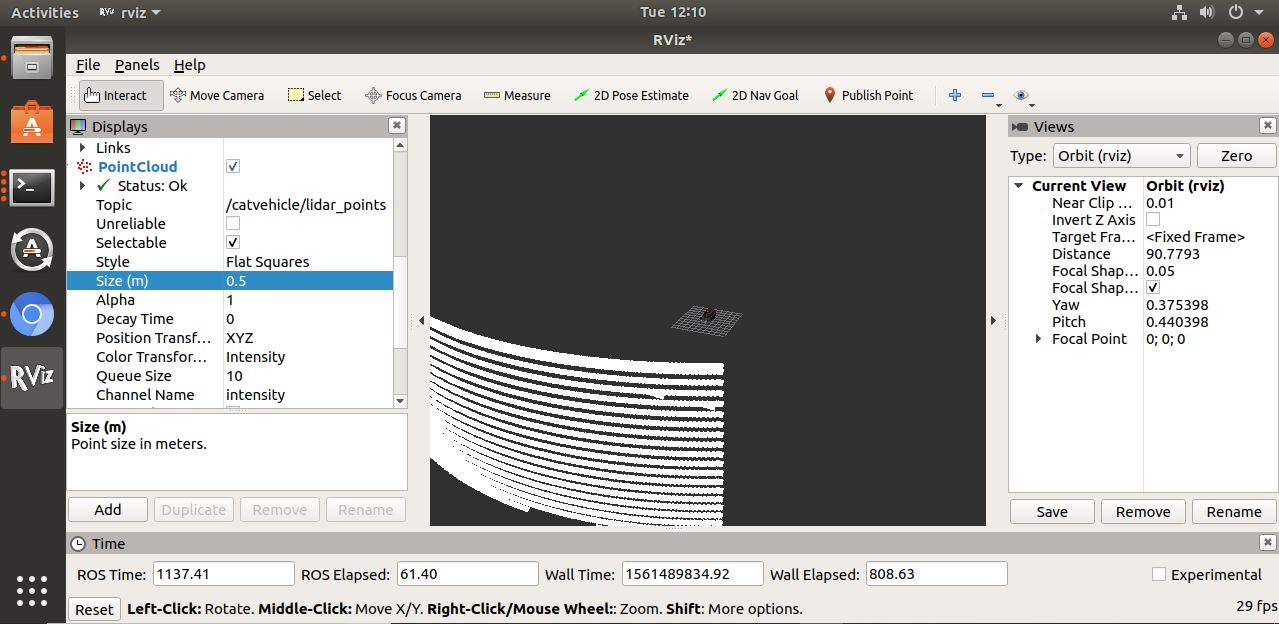
\includegraphics[scale=.3]{rviz1.JPG}
	\caption{RVIZ}
\end{center}
\end{figure}

-Followed tutorial on publishing to a node using python: 
"[ROS In 5 Minutes] 003 - How to create a ROS Publisher"

-Connected tutorial to catvehicle in src folder

-Created working publisher with catvehicle running in Gazebo

\begin{figure}[h]
\begin{center}
	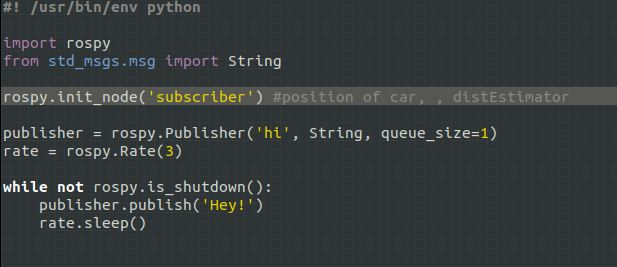
\includegraphics[scale=.6]{publisher1.JPG}
	\caption{Publisher}
\end{center}
\end{figure}

\section{Implementing simple reinforcement learning simulation week 4 6/26/2019}

-Attempting to add subscriber to recieve information from a catvehicle sensor and manipulate that with a publisher.

\begin{figure}[h]
\begin{center}
	\includegraphics[scale=.4]{positionSubscriber.JPG}
	\caption{Odometry information}
\end{center}
\end{figure}

-Succeeded in subscribing odometry information of the CAT vehicle

-Found out how to access position of any topic on python


\begin{figure}[h]
\begin{center}
	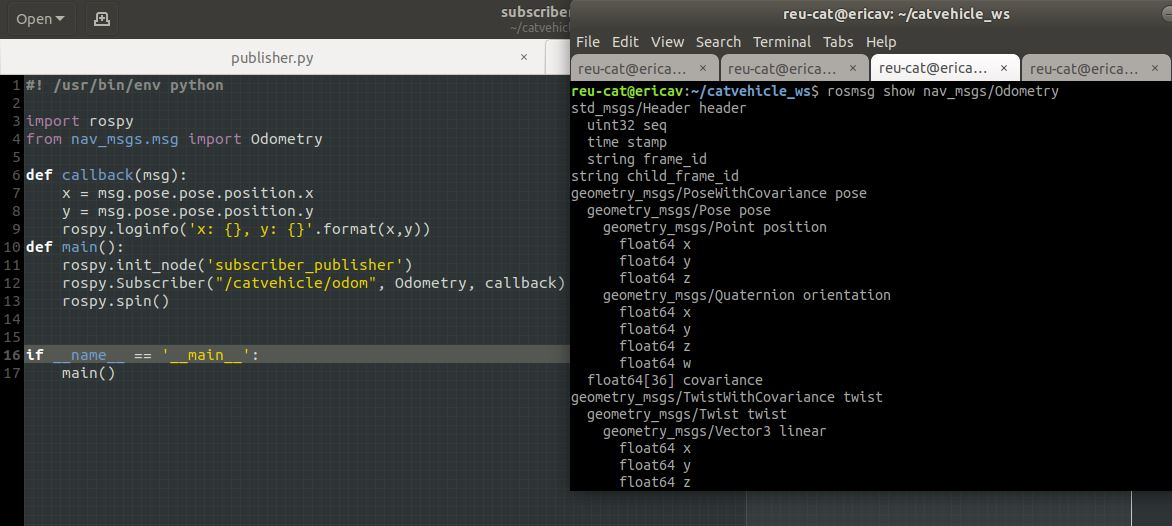
\includegraphics[scale=.5]{subscriberAndNav.JPG}
	\caption{topic position}
\end{center}
\end{figure}

\section{Implementing simple reinforcement learning simulation week 4 6/27/2019}

\begin{figure}[h]
\begin{center}
	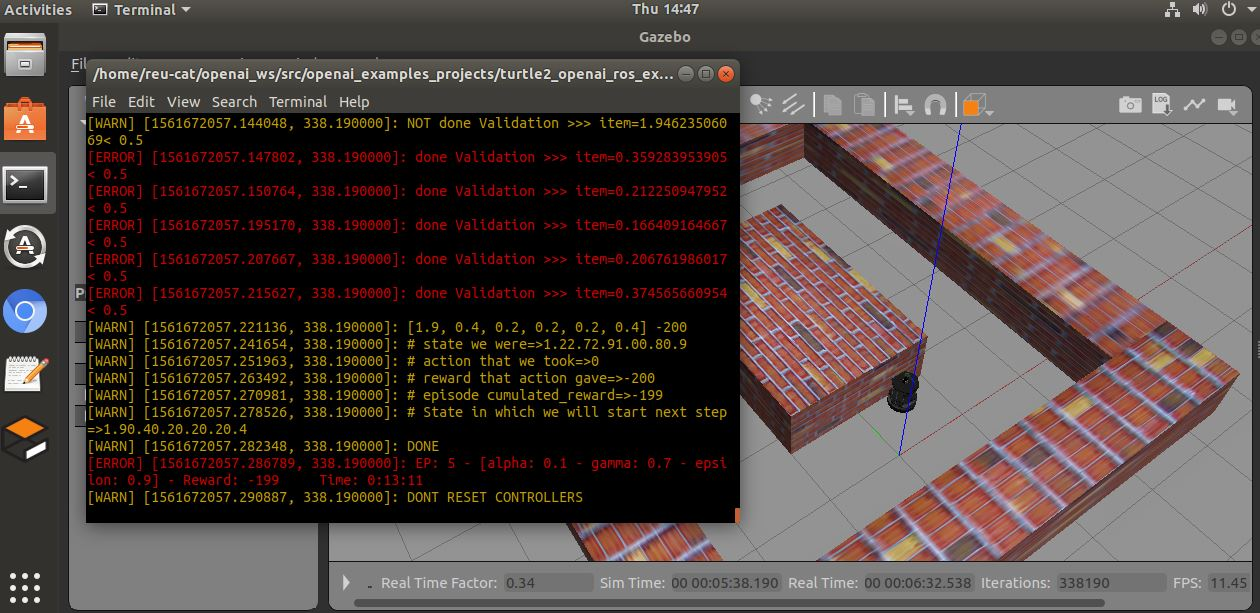
\includegraphics[scale=.3]{machinelearning1.JPG}
	\caption{openai working example}
\end{center}
\end{figure}

-Created an openai working example of reinforcement learning

\section{Implementing simple reinforcement learning simulation week 4 6/28/2019}

-Learn and deconstruct the reinforcement learning openai example for use in CAT Vehicle

\section{Implementing simple reinforcement learning simulation week 5 7/2/2019}

\begin{figure}[h]
\begin{center}
	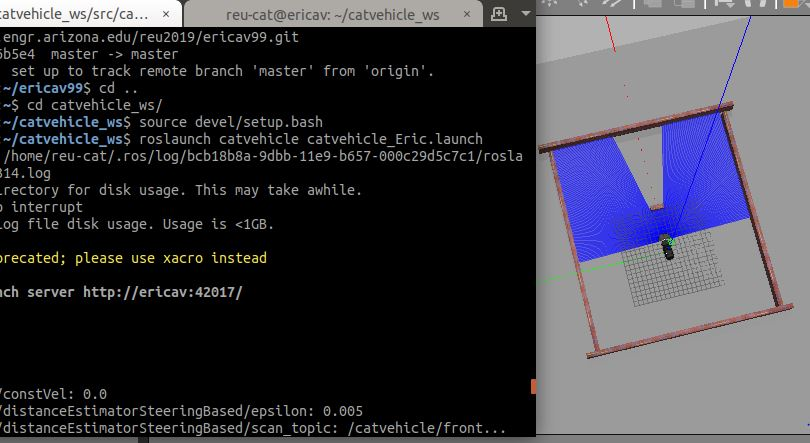
\includegraphics[scale=.5]{completesquare.JPG}
	\caption{openai enviroment for CAT Vehicle object collsion test}
\end{center}
\end{figure}

-Finished world for testing simple object collision

-Made draft for task enviroment and training script for openai in relation to the CAT Vehicle

\begin{figure}[h]
\begin{center}
	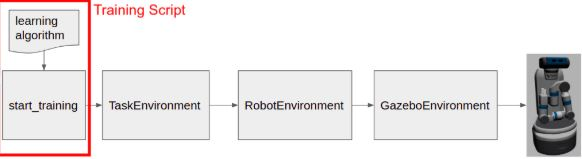
\includegraphics[scale=.5]{johnpic.JPG}
	\caption{openai and how it works with ROS and Gazebo}
\end{center}
\end{figure}

\section{Implementing simple reinforcement learning simulation week 6 7/8/2019}

-Plan to implement more worlds for training

\section{Implementing simple reinforcement learning simulation week 6 7/9/2019}

-Create a brick(person) moving in a world with the catvehicle

\section{Implementing simple reinforcement learning simulation week 6 7/9/2019}

-Created CAT vehicle moving across the reinforcement learning induced CAT Vehicle world

\begin{figure}[h]
\begin{center}
	\includegraphics[scale=.5]{personcat.JPG}
	\caption{CAT vehicle moving across the reinforcement learning induced CAT Vehicle world}
\end{center}
\end{figure}

\end{document}



